\chapter{Social Networks}

 The next day Rishnak was talking with his ghost friends about his mathematical adventures with Ajur. Seeing Ajur and Jura approach. Rishnak cut short his conversation with his friends and joined Ajur and Jura. Rishnak started the session, saying that over the last century, application of graph theory in fields like Engineering, Physics and Optimization Problems. Lately, however,  with the prolific use of social network applications such as Facebook, Twitter and Linked in, sociologists and psychologists have also found Graph Theory methods useful in their work.  
Stanley Milgram, a famous psychologist wanted to show that people are well connected. He devised an experiment wherein he selected a collection of people in midwestern United States and asked them to send post cards to a person in Boston. If they did not know the person then they could send the post card to a person that knows some one who knows the selected individual in Boston. The result of the experiment showed that most of the letters reached the destination individualin Boston in 5 or 6 steps. The experiments showed the diameter (longest of the shortest distance between vertices) of a social network is very small.

Social network has also been used in connection with a network of actors. Actors/Actresses form the vertices and vertices are adjacent if the corresponding actors/actresses have acted in the same film. There is an actor by the name of Kevin Bacon who has acted with a number of actors/actresses. Questions like what is your Kevin Bacon distance were answered using Social networks. It is essentially the length of the path  in the co-actor network. A dedicated website finds a path \url{http://oracleofbacon.org/movielinks.php} There is even a play about six degrees of separation. Again this shows the diameter of the network is very small and there is a vertex with a large degree (Kevin Bacon).

Social networks have also been used in co-author (of scientific and mathematical publications) networks. Paul Erd\H{o}s was a famous twentieth century mathematicians and a prolific contributor to Graph Theory was . He had written many papers with a many different  co-authors. Authors become vertices and two vertices (authors) are connected by an edge if they have written a paper together. American Mathematical Society has a website that calculates Erd\H{o}s distance to authors
\url{https://mathscinet.ams.org/mathscinet/collaborationDistance.html}. Usually Erd\H{o}s distance to many graph theorists is a very small number because of the collaborative nature of the work and an author like Paul Erd\H{o}s has written a large number of papers with a large number of co-authors (vertex corresponding to Erd\H{o}s has a large degree).

 Social networks have been used to spread real news and abused to spread rumors and disinformation called fake news. The news (both real and fake news) about individuals or political parties can be spread or shared with
 one's friends and friends of friends and eventually with the entire network. Most of the fake news items or  generated by bots (or computer programs). Advancs in image and audio manipulation make it nearly impossible to distinguish between the real and fake 
 Rishnak mentioned that degree distribution of Social networks follow a powerlaw. See Figure \ref{21p1}.  There are a few vertices with large degrees and there are a lot of vertices with small degrees.  The vertices with large degrees have many adjacent vertices and they may be treated as popular persons.
 \begin{figure}
 \begin{center}
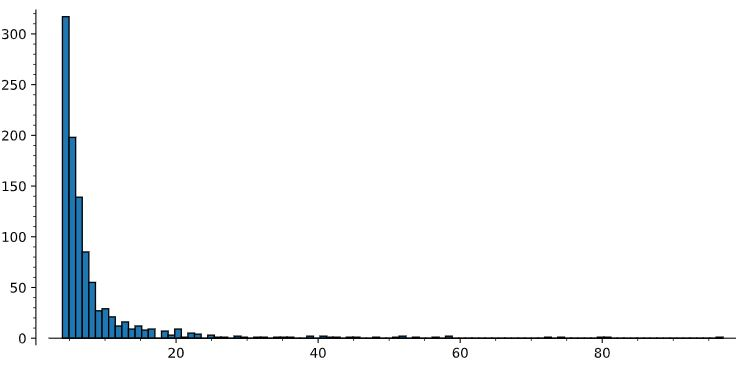
\includegraphics[width=0.8\textwidth]{degreepowerlawdist.jpg}
\caption{Degree Distribution of a social network}\label{21p1}
\end{center}

\end{figure}
\begin{newpage}
\end{newpage}
 
 Ajur remarked that Erd\H{o}s and Renyi model of random graphs seem to have a uniform degree distribution (that is all vertices have roughly the same degrees.
 
 Rishnak started with an example using facebook. Facebook graph consists users as vertices and there is an edge of two users if they are friends of each other (in facebook, friends is a symmetirc relation). It has been
 have found the average number of facebook friends per user (i.e., the average degree of a vertex) is 300 and the median degree is 200. The face book graph has roughly two billion vertices (man vertices could be fake users and some vertices could be groups). Median degree 200 means that a billion users have less than 200 friends. Facebook restricts that the maximum number of friends one can have is 5000. According to sociologists, a person can be close to at most 150 friends. Also facebook graph has an average separation or diameter of 3.74 \footnote{\url{https://research.fb.com/blog/2016/02/three-and-a-half-degrees-of-separation/}}
 
 There is a facebook paradox which states that most people have fewer friends than their friends have, on average. We can see this from the following example Figure \ref{21g1}.
 \begin{figure}
\begin{center}
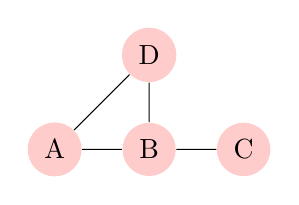
\begin{tikzpicture}
  [scale=.6,auto=left,every node/.style={circle,fill=red!20}]
  \node (n1) at (1,7) {A};
  \node (n2) at (3,7)  {B};
  \node (n3) at (5,7)  {C};
  \node (n4) at (3,9)  {D};

  \foreach \from/\to in {n1/n2,n2/n3,n2/n4,n1/n4}
    \draw (\from) -- (\to);

\end{tikzpicture}
\caption{ Graph explaining Facebook friends Paradox}\label{21g1}
\end{center}
\end{figure}

In this graph, average number of friends(average degree) is $\frac{2+2+3+1}{4}=2$.  A sees that D has 2 friends and B has 3 friends. B sees that A and D have 2 friends and C has 1 friend. C sees that B has 3 friends. D sees that A has 2 friends and B has 3 friends. Average number of friends one sees 
$\frac{2+3+2+2+1+3+2+3}{8}=2.25$. This is in contradiction to the common belief that one has more friends than their friends have!. Rishnak mentioned that there is a nice mathematical explanation for this phenomenon and that Ajur should discover it his own.

Kinaja, the ghost perked up and listened to the conversations between Rishnak and Ajur. She added that virtual social netwroks being unregulated do cause a lot harm and she listed the following points to Ajur (and to Rishnak).
\begin{enumerate}
    \item Users could be bullied.
    \item  Bots and trolls, pretending to be genuine users,  can propagate misinformation.
    \item  Ones private information gets stolen or sold to advertisers!
\end{enumerate}

Rishnak and Ajur agreed with Kinaja. That was a good place to stop the discussin and it was time to go home.